Elige la respuesta para cada pregunta, a partir de las imágenes de la figura \ref{fig:camionesdecarga01}.

\begin{multicols}{2}
    \begin{figure}[H]
        \centering
        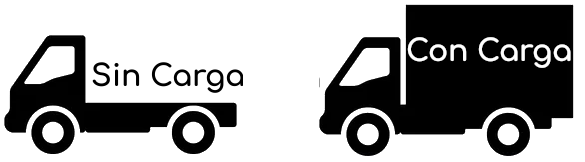
\includegraphics[width=0.8\linewidth]{../images/camionesdecarga01}
        \label{fig:camionesdecarga01}
        \caption{Representación de dos vehículos de carga.}
    \end{figure}

    \begin{parts}
        \part  ¿Cuál de ellos será más fácil poner en movimiento?

        \begin{oneparcheckboxes}\footnotesize%
            \choice El camión sin carga.
            \choice El camión cargado. \\
            \choice Los dos camiones requieren el mismo esfuerzo.
        \end{oneparcheckboxes}

        \part  Si ambos camiones se movieran a la misma velocidad,
        ¿a cuál de ellos le resultaría más fácil frenar?

        \begin{oneparcheckboxes}\footnotesize%
            \choice El camión sin carga.
            \choice El camión cargado. \\
            \choice Los dos camiones requieren el mismo esfuerzo.
        \end{oneparcheckboxes}

        \part  ¿Cuál podría aumentar más rápido su velocidad?

        \begin{oneparcheckboxes}\footnotesize%
            \choice El camión sin carga.
            \choice El camión cargado. \\
            \choice Los dos camiones aumentan su velocidad con la misma
            rapidez.
        \end{oneparcheckboxes}

        \part  ¿Cuál de los camiones podría tomar una curva con más
        facilidad si ambos se están moviendo a la misma velocidad?

        \begin{oneparcheckboxes}\footnotesize%
            \choice El camión sin carga.
            \choice El camión cargado. \\
            \choice Los dos camiones requieren el mismo esfuerzo.
        \end{oneparcheckboxes}

        \part ¿Cuál de ellos será más difícil poner en movimiento?
        \begin{oneparcheckboxes}\footnotesize%
            \choice El camión sin carga.
            \choice El camión cargado. \\
            \choice Los dos camiones requieren el mismo esfuerzo.
        \end{oneparcheckboxes}

        \part ¿Cuál podría aumentar más lento su velocidad?

        \begin{oneparcheckboxes}\footnotesize%
            \choice El camión sin carga.
            \choice El camión cargado. \\
            \choice Los dos camiones aumentan su velocidad con la misma rapidez.
        \end{oneparcheckboxes}

        \part Si ambos camiones se movieran a la misma velocidad,
        ¿a cuál de ellos le resultaría más difícil frenar?

        \begin{oneparcheckboxes}\footnotesize%
            \choice El camión sin carga.
            \choice El camión cargado. \\
            \choice Los dos camiones requieren el mismo esfuerzo.
        \end{oneparcheckboxes}

        \part ¿Cuál de los camiones podría tomar una curva con más
        dificultad si ambos se están moviendo a la misma velocidad?

        \begin{oneparcheckboxes}\footnotesize%
            \choice El camión sin carga.
            \choice El camión cargado. \\
            \choice Los dos camiones requieren el mismo esfuerzo.
        \end{oneparcheckboxes}

        \part Si se reduce la carga de arena de tal manera que la masa
        del camión sea la mitad de su masa inicial, mientras el conductor pisa el
        acelerador con la misma fuerza y mantiene el camión en la misma dirección,
        ¿qué pasa con la acelaración del camión?

        \begin{oneparcheckboxes}\footnotesize%
            \choice Aumenta al doble.
            \choice Disminuye a la mitad.\\
            \choice No cambia.
        \end{oneparcheckboxes}
        %\vspace{1cm}

        \part  Si el camión cargado va dejando gradualmente parte de su
        cargamento mientras el
        conductor pisa el acelerador con la misma fuerza y mantiene el camión
        en la misma dirección,
        ¿qué pasa con su rapidez?

        \begin{oneparcheckboxes}\footnotesize%
            \choice Aumenta.
            \choice Disminuye.
            \choice No cambia.
        \end{oneparcheckboxes}
    \end{parts}
\end{multicols}